Ahogy azt a Green-függvények bevezetésénél említettük, alkalmasak a (lokális) állapotsűrűség meghatározására \cite[7. o.]{economou2006green},
\begin{equation}
	\rho\left(E\right) = -\frac{1}{\pi}\lim_{\epsilon \to 0^+} \Im\Tr\op{G}\left(E + i\epsilon\right),
	\label{green:densityeq}
\end{equation}
\begin{equation}
	\rho(x,E)=-\frac{1}{\pi}\lim_{\epsilon\to 0^+}\Im G(x,x,E+i\epsilon).
	\label{green:localdensityeq}
\end{equation}
Az állapotsűrűség $\rho(E)\,dE$ az állapotok száma egy $dE$ energiatartományban. $\rho(x,E)\,dE\,dx$ pedig a megtalálási valószínűséggel súlyozott állapotok száma $dx$ intervallumban $dE$ energiatartományban, az úgynevezett lokális állapotsűrűség.

Ezeket a formulákat numerikus módon közelítőleg ki lehet értékelni kicsi, de véges $\epsilon$ választásával, ezt szemlélteti \aref{green:állapotsűrség}. ábra.
\begin{figure}[H]
	\centering
	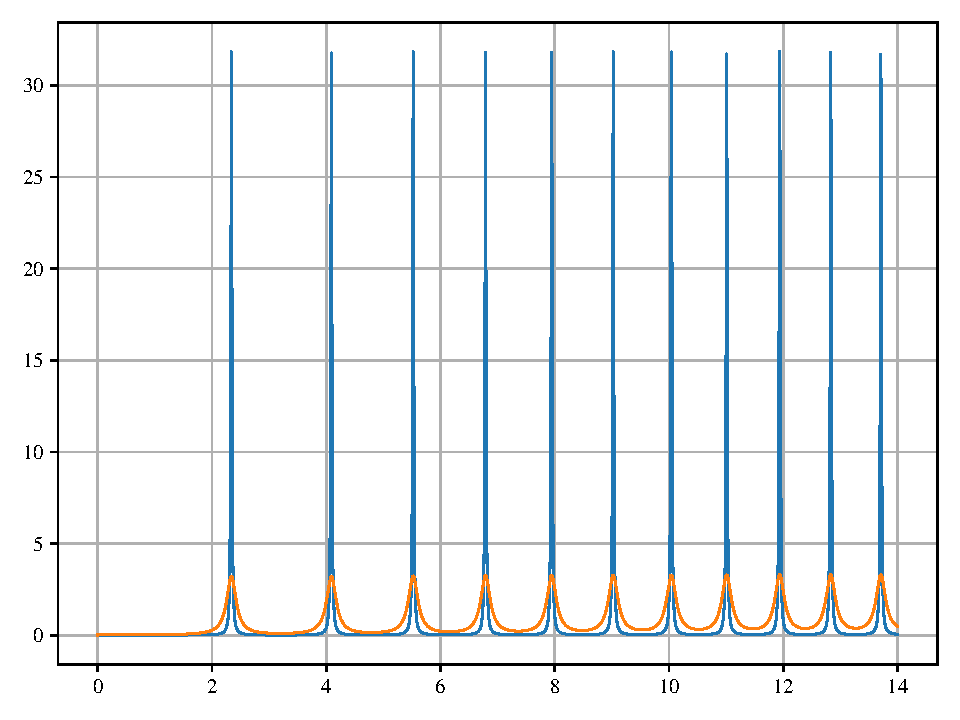
\includegraphics[scale=1]{./figs/dosfromgreen.pdf}
	\caption[Állapotsűrűség]{\Aref{green:densityeq}. képlet alapján számolt állapotsűrűség. A kék függvényt $b\epsilon = 0.1$, a narancssárga görbét pedig $b\epsilon = 0.01$ helyettesítéssel kaptuk. Látható, hogy $\epsilon$ csökkentésével a tüskék egyre keskenyebbek, és egyre magasabbak lesznek.}
	\label{green:állapotsűrség}
\end{figure}
Ennek a közelítésnek egy jó tulajdonsága, hogy a formula származtatásához a jól ismert
\begin{equation}
	\frac{1}{x\pm i\epsilon} = \frac{1}{x}\mp i\pi\delta(x)
\end{equation}
formulát lehet használni. Ennek a formulának a levezetése során a $\delta(x)$ állandó területű, de egyre szűkebb Lorentz-görbék határértékeként bukkan fel. Ez azt jelenti, hogy véges $\epsilon$ esetén is a sajátenergiákhoz tartozó csúcsok alatti terület változatlan, az állapotsűrűség $E$ szerinti integrálja nagy $E$-k és véges $\epsilon$ esetén is pontos marad.
\begin{figure}[H]
	\centering
	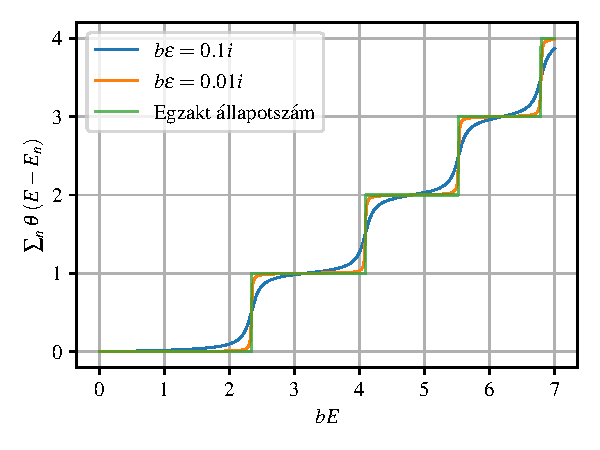
\includegraphics[scale=1]{./figs/numberofstatesfromgreen.pdf}
	\caption[Állapotok száma]{\Aref{green:állapotsűrség}. ábrán bemutatott függvények integrálja látható ezen az ábrán. Mind a két függvény ugrása közelítőleg $1$, ami at jelenti, hogy \aref{green:állapotsűrség}. ábrán látható tüskék alatti terület jó közelítéssel $1$. Az $\epsilon$ csökkentése a lépcsőfüggvényhez közelíti az integrált függvényt, ami egyezik az elvárásokkal és \aeqref{green:densityeq} egyenlettel.}
\end{figure}
\Aeqref{limits:semiinfinite} Green-függvényhez tartozó állapotsűrűség kvalitatíve nem különbözik az előző számítás menetétől és eredményétől, hiszen az előzőhöz hasonlóan csak diszkrét sajátenergiák vannak, ezeknek csupán az értékük különböző.

Más a helyzet \aeqref{limits:nowallgreen1}, \eqref{limits:nowallgreen2} Green-függvénnyel. Itt csak folytonos spektrumba tartozó sajátenergiák vannak, mind szórásállapotokhoz tartoznak. Ebben az esetben csak a lokális állapotsűrűséget lehet értelmezni, hiszen a sajátállapotok négyzetének integrálja végtelen, csak Dirac-deltára normálhatóak. \Aeqref{green:localdensityeq} egyenletnek megfelelően a határérték kiszámításához a pozitív képzetes részre vonatkozó \eqref{limits:nowallgreen1} kifejezést kell használni,
\begin{dmath}
	\rho(x,E)=-\frac{1}{\pi}\lim_{\epsilon\to 0^+}\Im\left\lbrace\frac{a^2\pi}{F}\Ai(ax-b(E+i\epsilon))\Bigl(\Bi(ax-b(E+i\epsilon))-i\Ai(ax-b(E+i\epsilon))\Bigr)\right\rbrace=\frac{a^2}{F}\Ai^2(ax-bE).
\end{dmath}
Nem meglepő módon ez az $E$ energiájú sajátállapot abszolútérték négyzete \eqref{nowell:sajátfüggvény}. A nomálási faktor is egyezik, hiszen $\frac{a^2}{F}=ab$.




















